\documentclass[11pt,a4paper]{article}
\usepackage[utf8]{inputenc}
\usepackage[italian]{babel}
\usepackage{amsmath}
\usepackage{amsfonts}
\usepackage{amssymb}
\usepackage{graphicx}
\usepackage{caption}
\usepackage{subcaption}
\author{Volpini, Paganini, Finazzer, Beghini}
\title{Effetto termoionico ed energia di Ionizzazione }
\begin{document}
\maketitle 
\section{Abstract}
Nella prima parte di questa esperienza si vuole studiare il fenomeno di produzione di correnti elettroniche per effetto termoionico in una camera da vuoto; si verificano sperimentalmente le leggi di Richardson e di Child. Nella seconda parte si studia invece il processo di ionizzazione di gas residui nella camera da vuoto; sperimentalmente si vogliono misurare le diverse energie di ionizzazione di alcune specie di gas.  
\section{Apparato sperimentale}

Come si evince dalla figura le principali componenti dell'apparato sperimentale sono:

\begin{figure}[!h]
  \begin{subfigure}[b]{0.6\textwidth}
    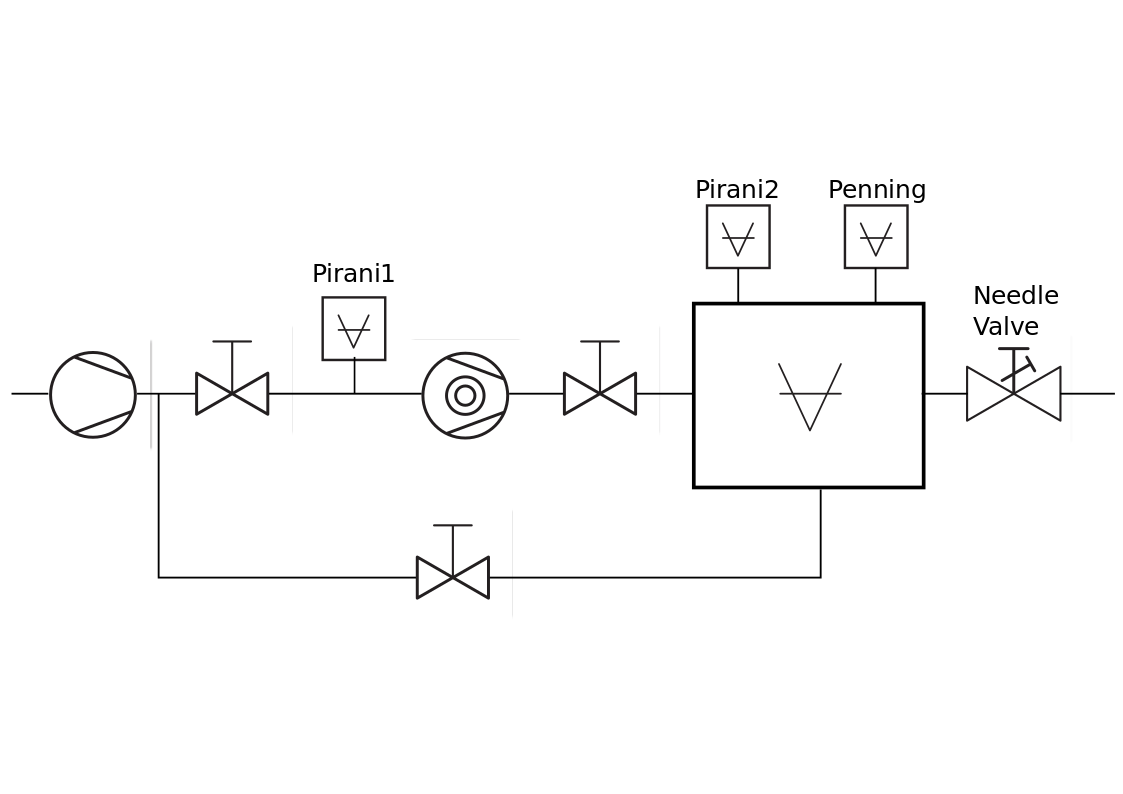
\includegraphics[width=\textwidth]{vuoto}
    \caption{schema apparato da vuoto} %eliminare intera riga se non si vuole didascalia
    \label{fig:f1}
  \end{subfigure}
  \hfill
  \begin{subfigure}[b]{0.4\textwidth}
    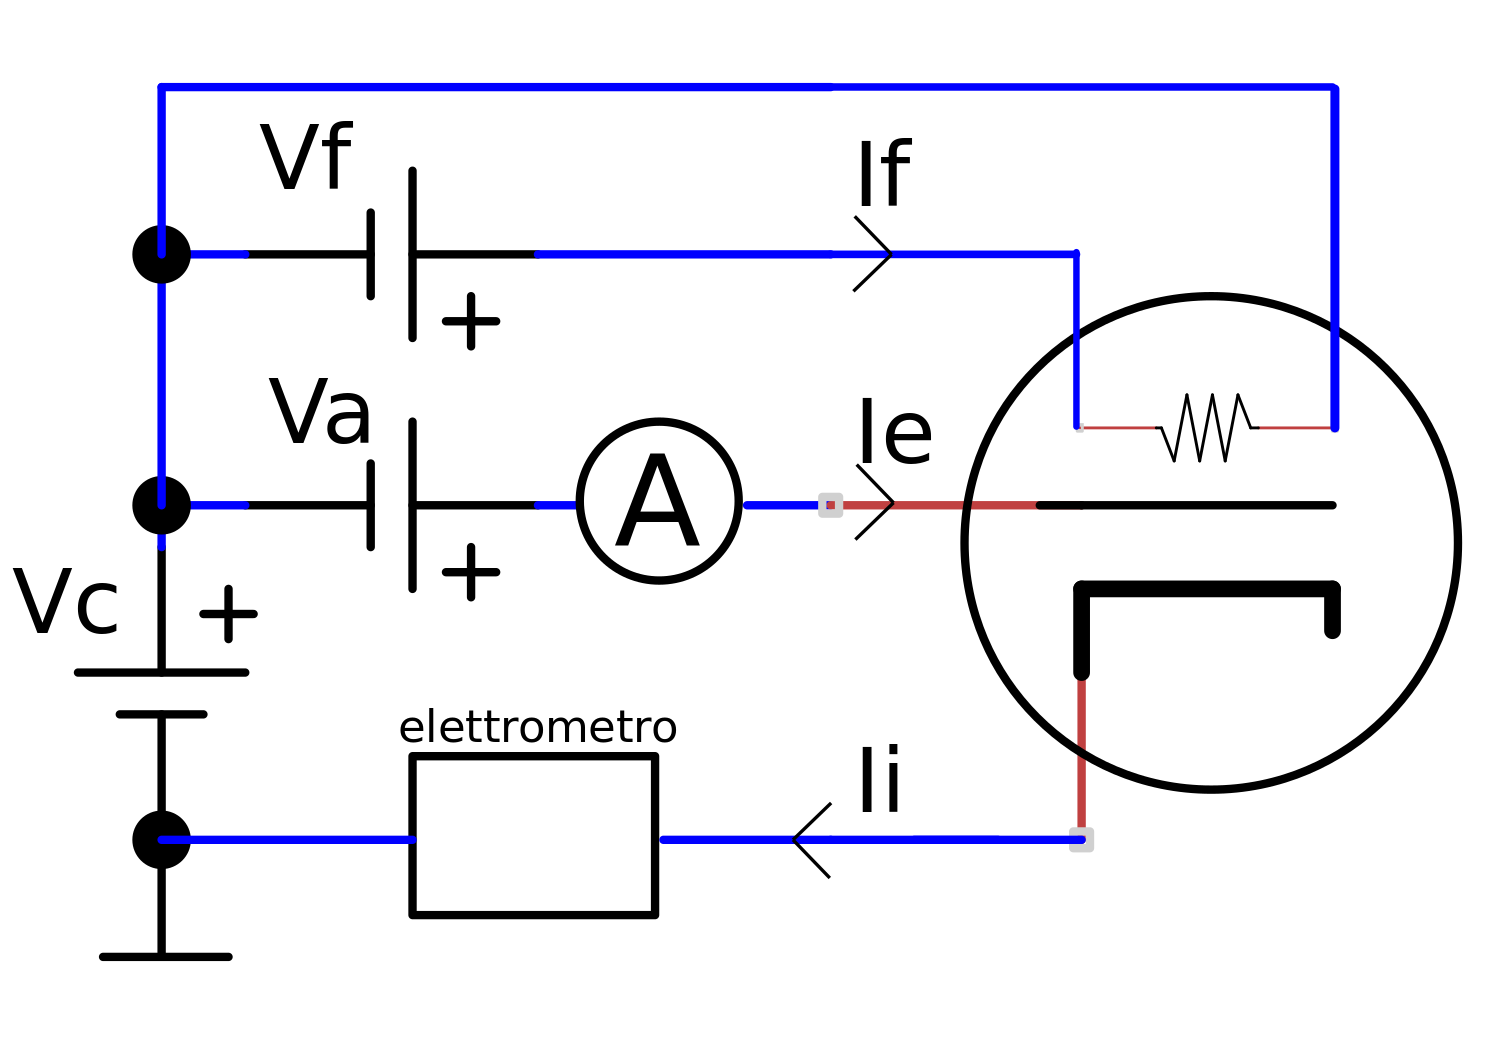
\includegraphics[width=\textwidth]{elettrico}
    \caption{schema circuito elettrico} %eliminare intera riga se non si vuole didascalia
    \label{fig:f2}
  \end{subfigure}
  %\caption{bla bla bla bla} %eliminare intera riga se non si vuole didascalia
\end{figure}

\begin{itemize}
\item camera da vuoto
\item misuratori di pressione Pennig (catodo freddo) e Pirani
\item pompa rotativa e pompa turbo-molecolare
\item valvola termoionica con filamento di tungsteno
\item generatori di corrente, elettrometro, multimetri digitali e palmari 
\end{itemize} 

\section{Prima parte}
Si comincia generando il vuoto all'interno della camera. Si utilizzano pompa rotativa e pompa turbomolecolare per raggiungere la pressione ($P\sim10^{-6} mbar$).

Instauriamo una differenza di potenziale ai capi del filamento collegandone gli estremi rispettivamente uno a massa ed uno ad un generatore; in questo modo è possibile riscaldare il filamento fino al raggiungimento di temperature tali da provocarne l'effetto termoionico. Il secondo generatore si usa invece per generare una differenza di potenziale tra filamento e anodo, e catturare quindi gli elettroni che si liberano dal filamento.

\subsection{Dati sperimentali}

Utilizziamo un filamento campione per calcolare la resistività del filamento utilizzato nella valvola termoionica $\rho=R_{s}\pi (d/2)^{2})/l_{s}=(6.5\pm 0.4)*10^{-8} \Omega m$. Tale valore risulta essere compatibile nell'ordine di grandezza con il valore presente in letteratura.

A questo punto è possibile calcolare la resistenza del filamento inserito nella valvola e soggetto ad effetto termoionico: $ R_{fil}=l_{fil}\rho/\pi (d/2)^{2})=(0.037\pm0.006) \Omega$. Dobbiamo a questo punto considerare il contributo alla resistenza dato dai cavi utilizzati per il circuito in esame: calcoliamo la resistenza dei cavi mediante la relazione $R_{cavi}=R_{tot}-R_{fil}$(modalità "4 wire" del multimetro). Supponendo che tali cavi non si riscaldino durante l'esperienza siamo in grado di separare i diversi contributi nel calcolo della resistenza $R_{tot}=R_{cavi}+R_{fil}$.

Successivamente si procede ad una stima della temperatura raggiunta dal filamento sottoposto ad effetto termoionico. La letteratura scientifica fornisce la seguente relazione $\dfrac{r_{fil}}{R_{T300k}}=\alpha \Delta T $. Invertendo la relazione stimiamo la temperatura finale del filamento.

Verifichiamo la legge di Richardon che studia l'andamento della corrente degli elettroni prodotti per effetto termoionico in funzione della temperatura del filamento. Misuriamo valori di corrente elettronica al variare del potenziale di filamento ($V_{fil}$) e quindi della temperatura dello stesso.



Grafichiamo il logaritmo del rapporto tra corrente elettronica e quadrato della temperatura rispetto all'inverso della temperatura. Tramite regressione lineare calcoliamo la funzione lavoro: $W = (8.2 \pm 3.5) eV$. La letteratura fornisce $\approx 4.32 \; - \; 5.22 \; eV$, valore compatibile con quello sperimentale.

	

Studiamo l'andamento della corrente elettronica in funzione del potenziale dell'anodo, concentrandoci nel range a bassi potenziali per verificare la legge di Child. 

\begin{figure}[!h]
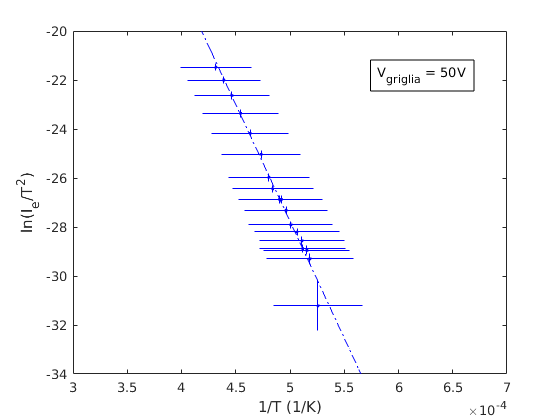
\includegraphics[width=\textwidth]{richardsonlin}
\end{figure}

In figura riportiamo i dati sperimentali con relativi fit; i parametri ottenuti da tali fit sono riportati in tabella.

\begin{center}
\begin{tabular}{|r|c|c|c|c|c|}
\hline

&\multicolumn{5}{|c|}{Temperature (K)}\\ \hline
&2406 $\pm$ 360& 	2318 $\pm$ 386&	2363 $\pm$ 393 &	2269 $\pm$ 377&	2238 $\pm$ 167\\ \hline
intercetta&	1.6&	0.7&	0.9&	0.4&	1.2\\ 
$[F C^{1/2} m^{-3/2}] \times 10^{-5}$&	$\pm$ 0.2&	$\pm$ 0.1&	$\pm$0.1&	$\pm$0.1&	$\pm$0.1	  \\ \hline
pendenza&	1.2 $\pm$ 0.1	&	1.6 $\pm$ 0.3&	1.5 $\pm$ 0.1&	1.6 $\pm$ 0.5&	1.5 $\pm$ 0.1\\ \hline 
\end{tabular}
\end{center}

I valori di pendenza corrispondono all'esponente del potenziale. La regressione lineare restituisce valori confrontabili entro un sigma con il valore teorico 3/2. I valori delle temperature hanno un grosso errore che è dovuto principalmente dalla poca accuratezza nel misurare la lunghezza del filamento e la sua resistenza.

\begin{figure}[h]
%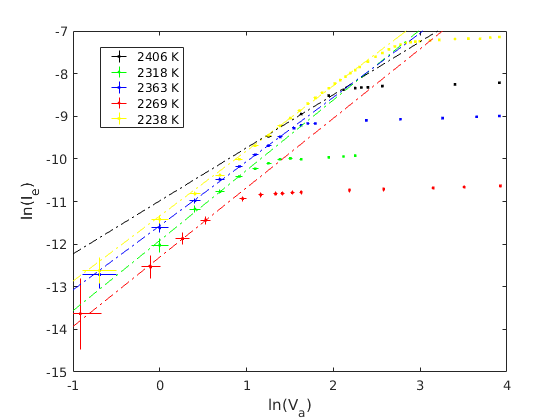
\includegraphics[scale=0.8]{child}
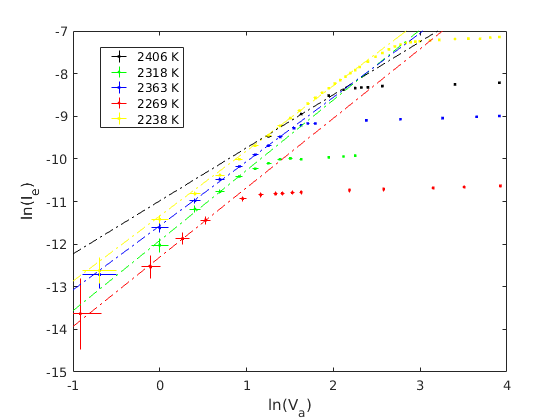
\includegraphics[width=\textwidth]{child}
\end{figure}

\newpage
\section{Seconda Parte}
 
In questa seconda parte dell'esperienza studiamo il fenomeno di ionizzazione di alcune specie di gas. Colleghiamo anche il collettore della valvola termoionica; in questo modo raccoglieremo gli atomi ionizzati sulla griglia esterna e ne potremmo misurare la corrente ionica. 

\subsection{Dati sperimentali}

Si verifica che all'aumentare della pressione nella camera da vuoto aumenti anche la corrente ionica misurata; questo è dovuto al fatto che aumentando la pressione in camera aumentiamo il numero di atomi della specie di gas e aumentiamo quindi il numero di atomi che possono essere ionizzati dagli elettroni.

Successivamente studiamo l'andamento della corrente ionica in funzione del potenziale di anodo. Si sottolinea che aumentando il potenziale di anodo aumenta anche la corrente elettronica prodotta per effetto termoionico; si provvede quindi ad effettuare una normalizzazione che permetta di considerare solo il contributo dell'energia degli elettroni bombardanti e non del loro numero (sull'asse delle ordinate del grafico si riporta quindi il rapporto $I_{i}/I_{e}$).

In ascissa del grafico troviamo la differenza di potenziale applicata all'anodo $V_{a}$ che risulta proporzionale all'energia cinetica degli elettroni. Finché tale energia non è sufficiente a ionizzare il gas non si misurano correnti ioniche mentre una volta superata tale energia soglia la corrente $I_{i}$ cresce. Eseguendo un fit lineare possiamo stimare il valore $V_{a}$ tale per cui $I_{i}$ è diversa da zero e ottenere quindi l'energia minima di ionizzazione.

\begin{tabular}{|c|c|c|}
\hline 
Gas & Energia ionizzazione sperimentale & Energia ionizzazione teorica \\ 
\hline 
Elio & 22.9 $ \pm $0.2 eV & 24.6 eV \\ 
\hline
Azoto & 21.6 $\pm$  eV & 15.6 eV \\ 
\hline 
\end{tabular} 

I valori sperimentali ottenuti non risultano compatibili con i valori teorici riportati nella letteratura. Il principale fattore di incertezza risulta essere il fatto che la differenza di potenziale applicata al filamento genera una distribuzione di energie per gli elettroni; questo comporta l'assenza di una curva ben definita e di conseguenza forte imprecisione nel fit. 

\begin{figure}[h]
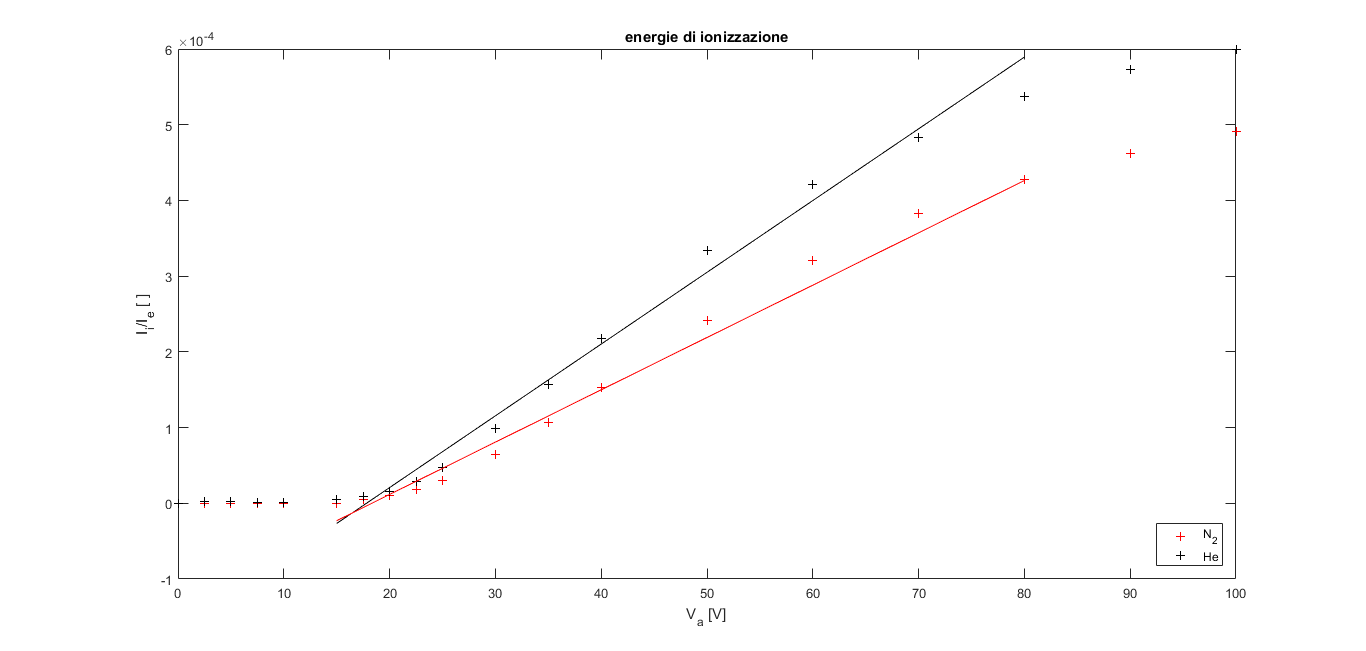
\includegraphics[width=\textwidth]{fig1}
\end{figure}

\end{document}
